\documentclass{beamer-control}
\usepackage{beamer-control-singlefile}
\INCLUDEONLY{Nonlinear Effects}
\begin{document}
\CONCEPT{Nonlinear Effects}

\begin{SUMMARY}
\begin{itemize}
\item Nonlinearities
\end{itemize}
\vfill References:
\begin{itemize}
\item \astrom{§14.6}
\end{itemize}
\end{SUMMARY}



\SUBCONCEPT{Nonlinearities}

\begin{frame}{Limitations due to nonlinear effects}
\begin{itemize}
\item We have mostly looked at linear systems, however nonlinear effects must be considered during the design phase of control systems
\item Nonlinearities due to actuation limits, measurement noise, and friction will limit the performance of controllers
\end{itemize}
\end{frame}


\begin{frame}{Actuation limits}
	\begin{itemize}
		\item Many systems have limits to their actuation --- limited torque from motors, maximum throttle, maximum flow rate through a pump
		\item These limits result in restrictions on the amplitude and rate of change of the control signal (or of internal state variables)
	\end{itemize}
\end{frame} 


\begin{frame}{Actuation limits - Example}
	\begin{itemize}
		\item Consider a servo system, where the actuator is a current-driven voice coil modelled by
		\[m\frac{\mathrm{d}^2x}{\mathrm{d}t^2}=F=k_I I\]
		where $m$ is the mass of the system, $x$ is the position of the mass, $F$ is the force, $I$ is the current, and $k_I$ is the motor constant
		\item The maximum acceleration $a_{\text{max}} =F_{\text{max}}/m=k_I I_{\text{max}}/m $ is given by the maximum current
		\item There is also a maximum velocity for a voice coil drive, $v_{\text{max}}=V_{\text{max}}/k_I$ given by the maximum voltage
	\end{itemize}
\end{frame} 



\begin{frame}{Actuation limits - Example}
	\begin{itemize}
		\item The problem of moving the mass from one position to another in minimum time is dependent on if the velocity is saturated or not
		\item Without velocity saturation, we can simply apply the maximum acceleration until the midpoint and then apply maximum deceleration
		\item For a scenario with velocity saturation, we are additionally limited by the maximum velocity which increases the minimum time
		\item The minimum time for a transition over a distance $l$ with zero velocity at start and end is
		\[t= \begin{cases}2 \sqrt{\ell / a_{\max }} & \text { if } \ell \leq v_{\max }^2 / a_{\max } \\ \ell / v_{\max }+v_{\max } / a_{\max } & \text { if } \ell>v_{\max }^2 / a_{\max }\end{cases}\]
	\end{itemize}

\end{frame} 

\begin{frame}{Actuation limits - Example}
\begin{figure}
	\vspace{-0.5cm}
	\centering
	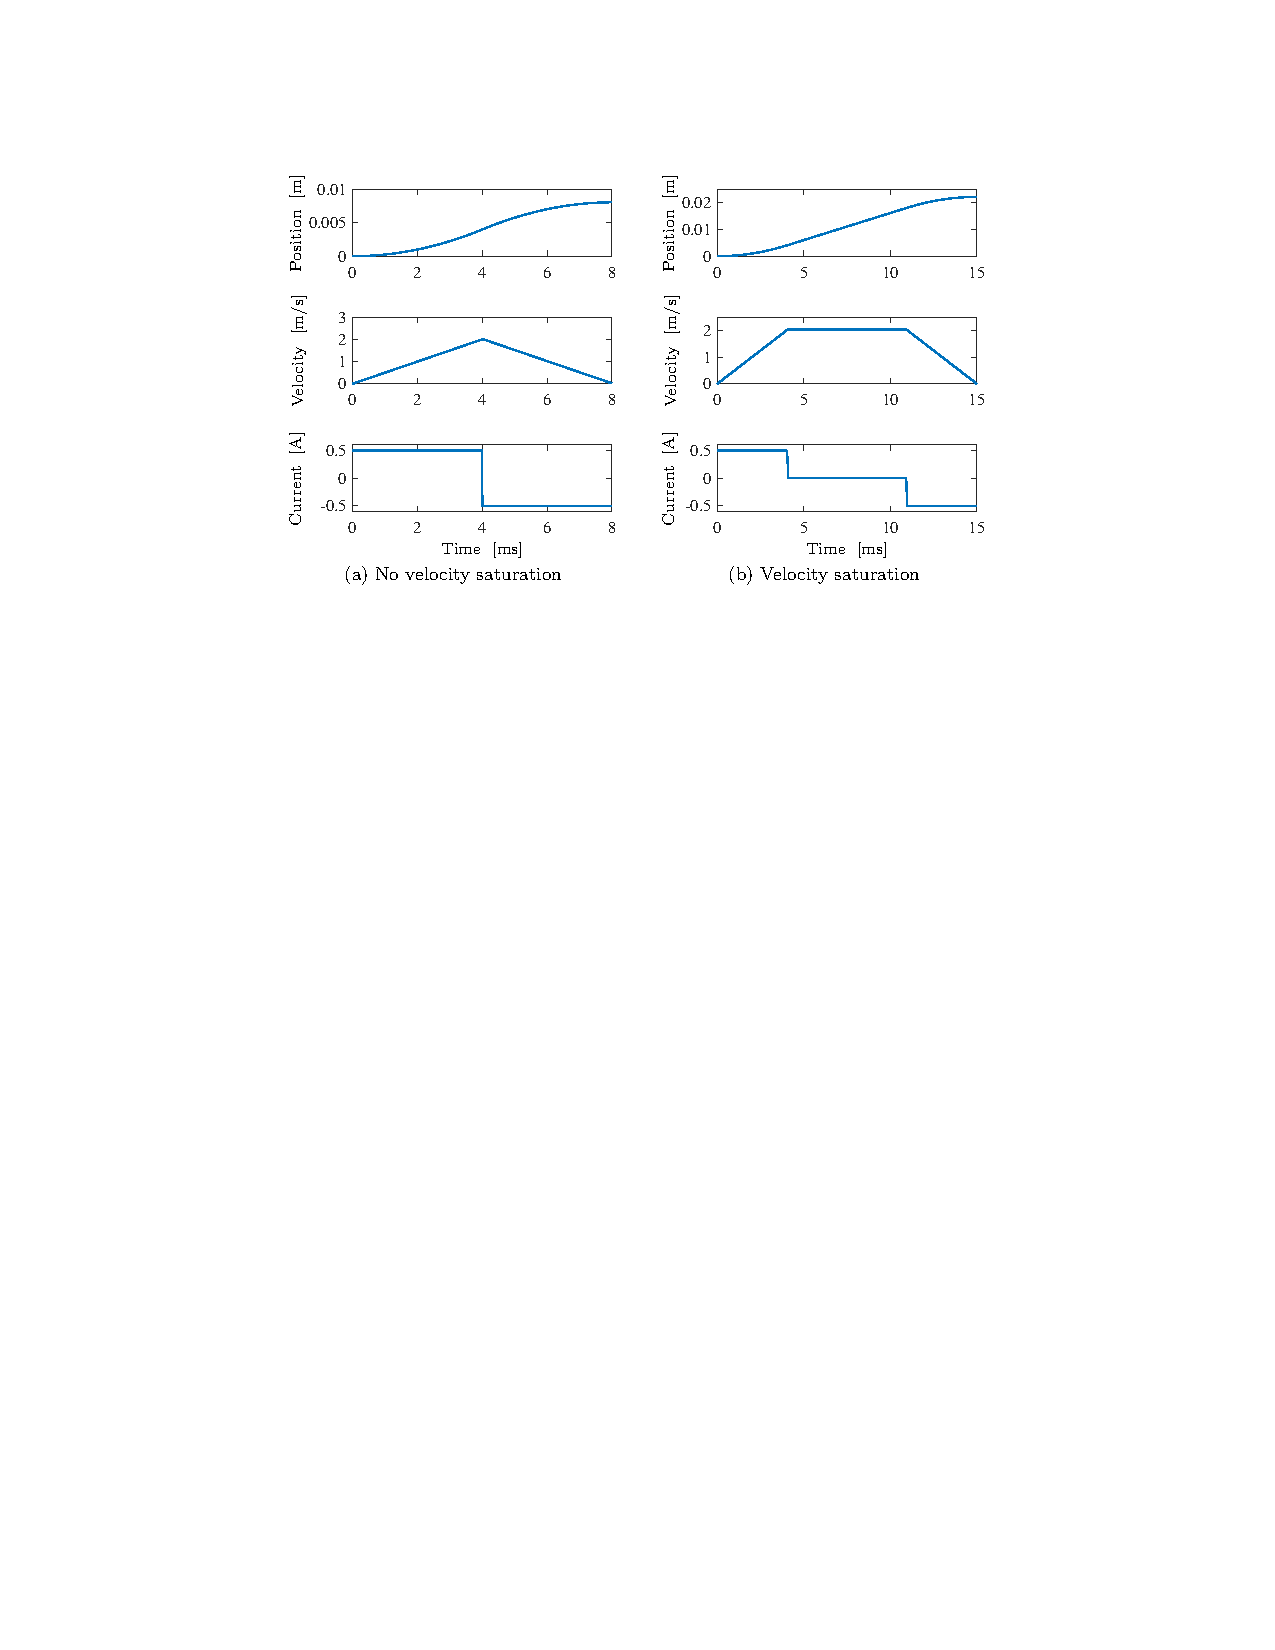
\includegraphics[width=10cm]{figure14.12}\\
	\vspace{-0.2cm}
	\textbf{Figure 14.12:} Minimum time transition for a servo system.
\end{figure}
\end{frame}

\begin{frame}{Measurement noise and friction}
\begin{itemize}
\item Measurement noise in the form of sensor noise, electronics, transmission equipment, and A/D and D/A converters results in fluctuations in the control signal
\item These fluctuations cause wear or saturation of the actuator
\item Friction is an inherently nonlinear phenomenon and may also generate oscillations that limit the closed loop performance
\end{itemize}
\end{frame}



\begin{frame}{Friction - Example}
	\begin{itemize}
		\item Consider the cart-pendulum balance system with state feedback but including a friction force given by
		\[F=-\mu_f M_t g \operatorname{sgn}(v)\]
		\item Experiments often show that friction on the cart creates oscillaiton
	\end{itemize}
	
\begin{figure}
	\vspace{-0.5cm}
	\centering
	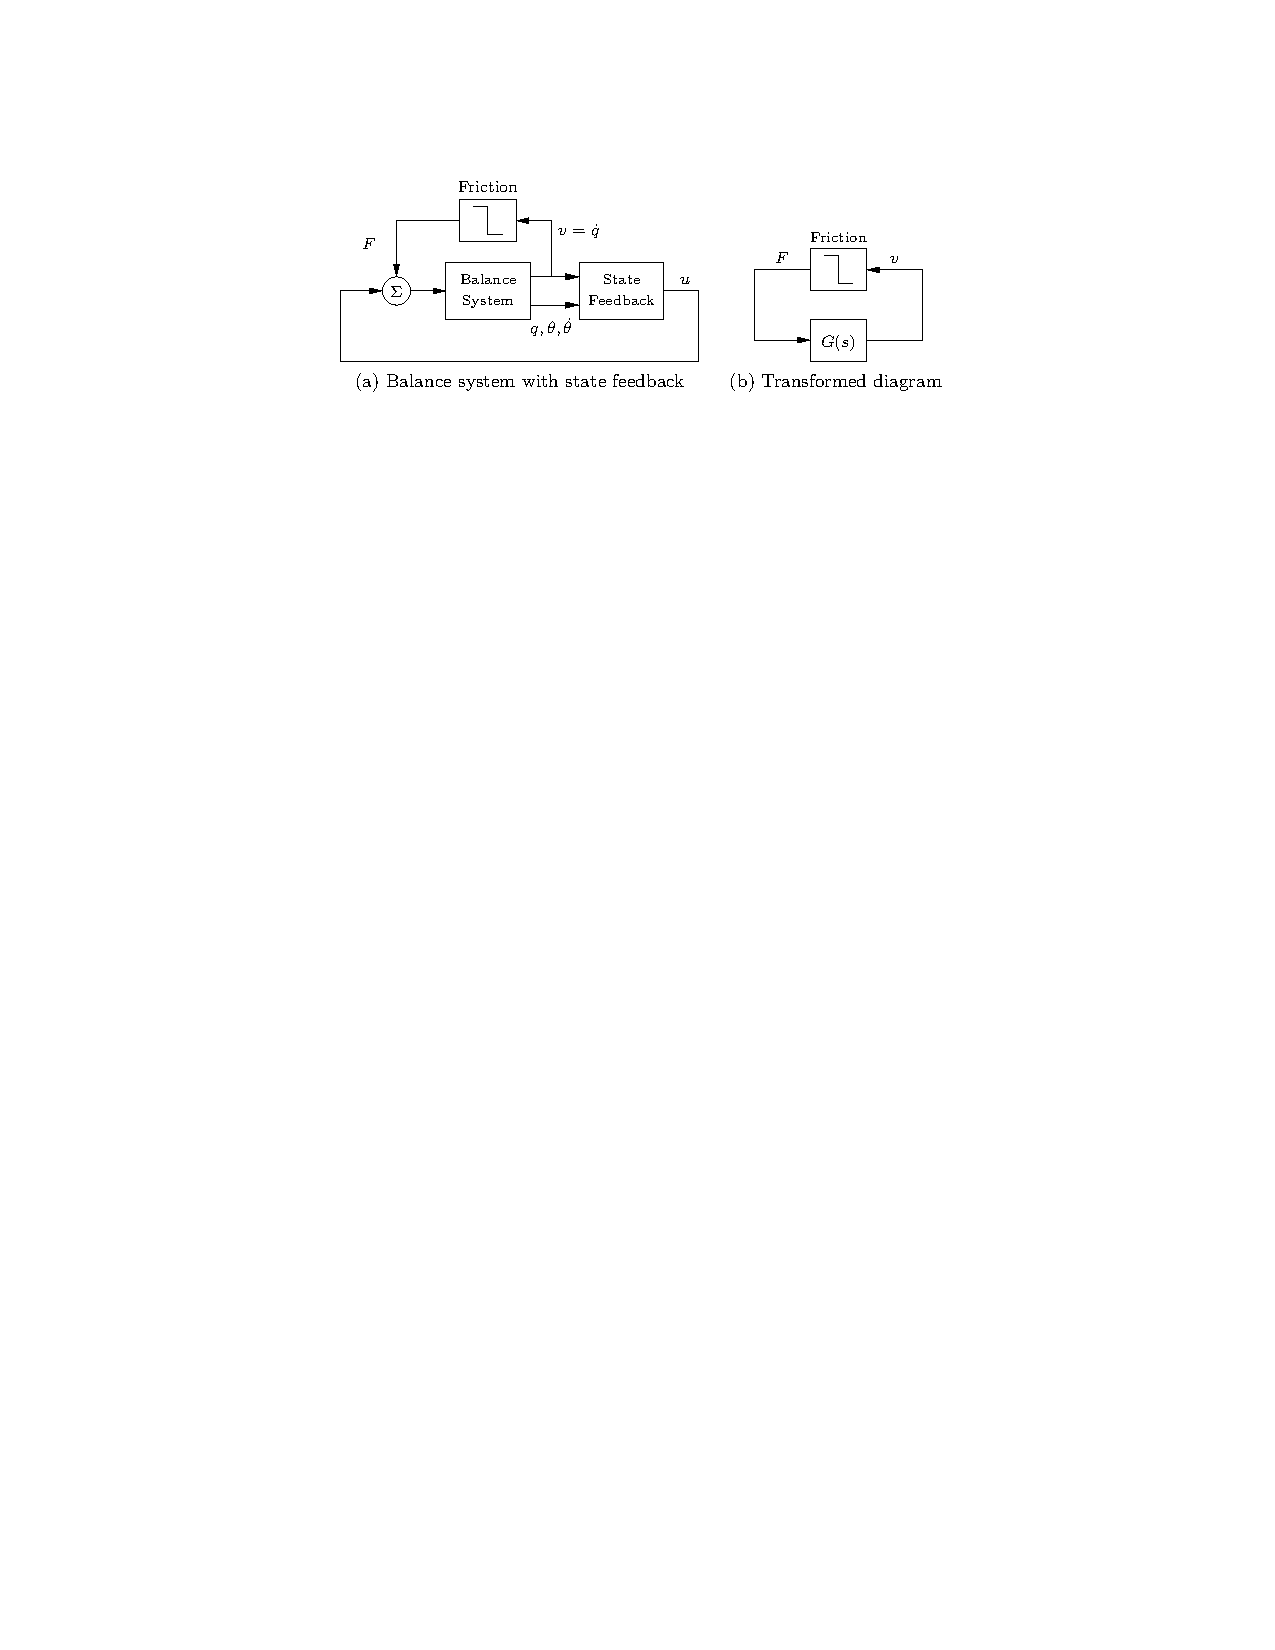
\includegraphics[width=10cm]{figure14.13}\\
	\vspace{-0.2cm}
	\textbf{Figure 14.13:} Block diagrams of a balance system with state feedback and friction.
\end{figure}
\end{frame}


\begin{frame}{Friction - Example}
	\begin{itemize}
		\item The results of a simulation of the system are shown below
	\end{itemize}
	
	\begin{figure}
		\vspace{-0.5cm}
		\centering
		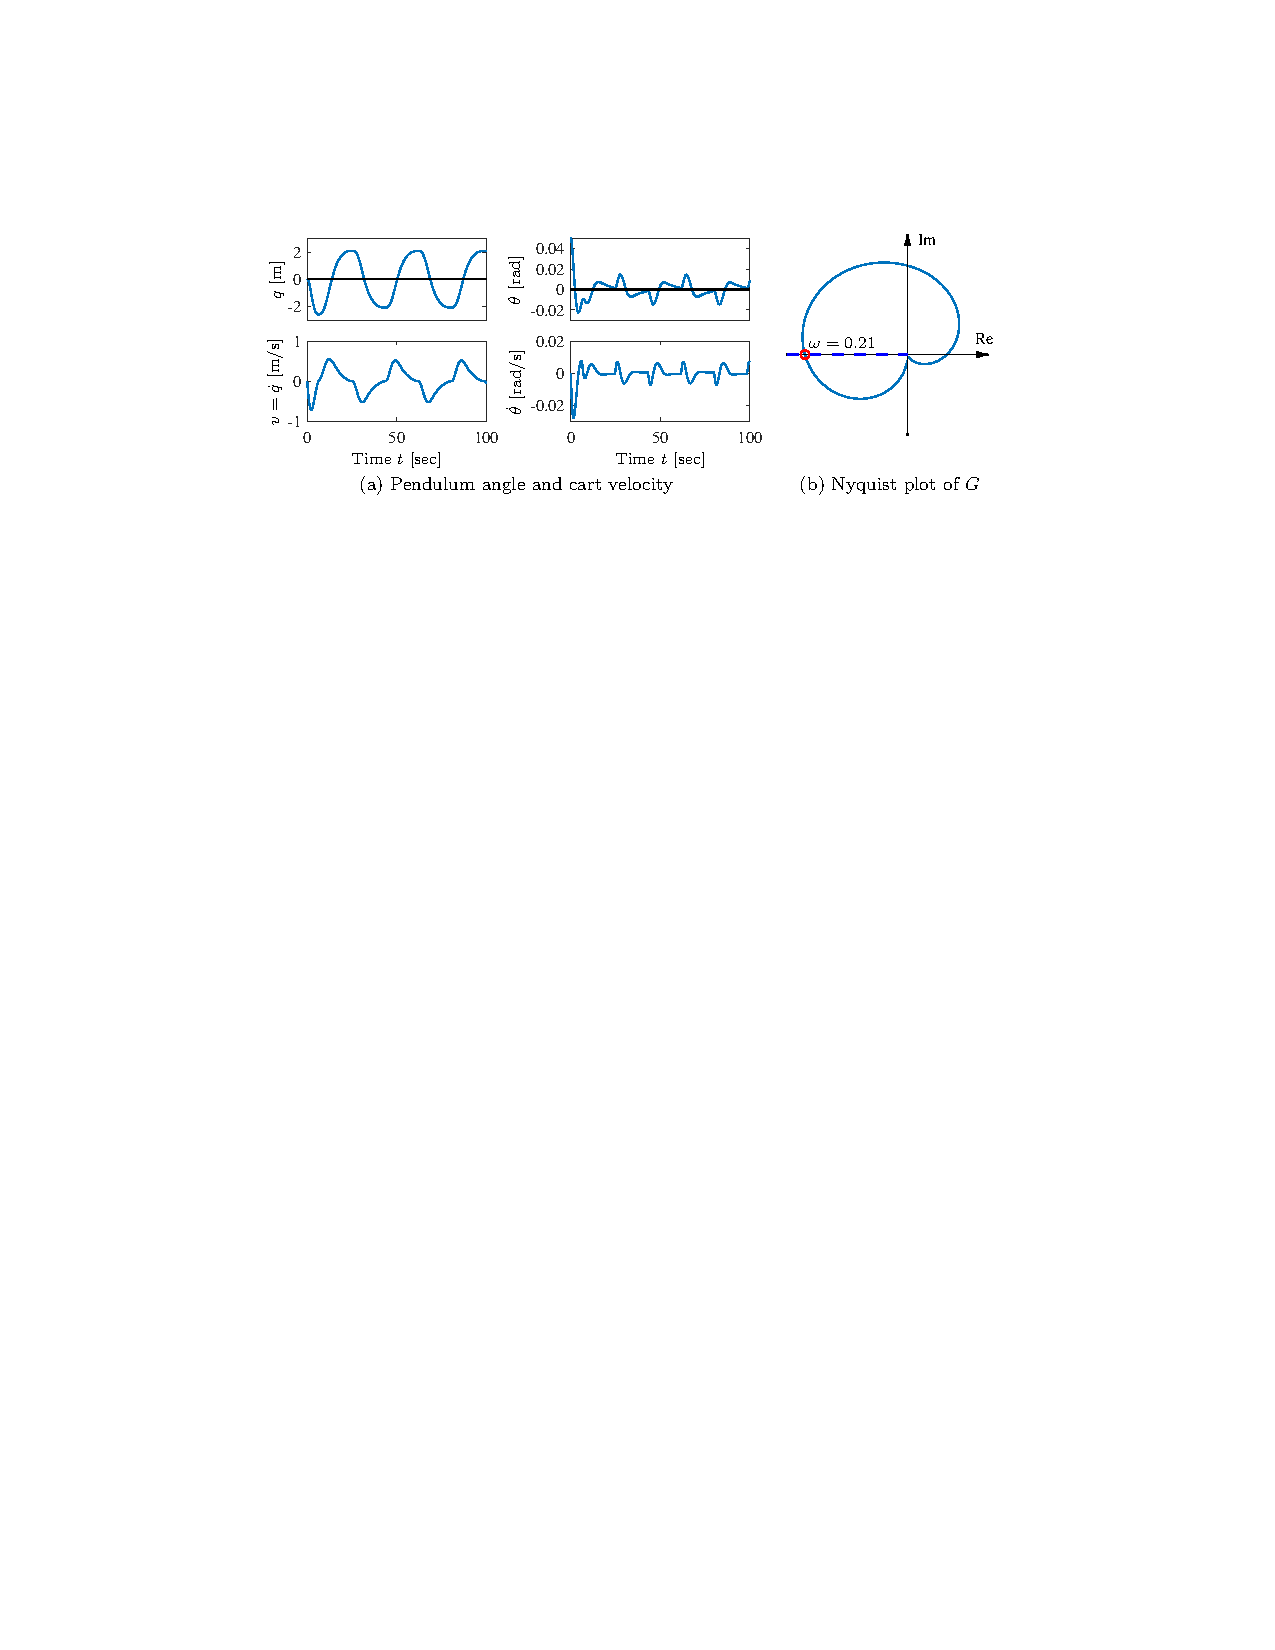
\includegraphics[width=10cm]{figure14.14}\\
		\vspace{-0.2cm}
		\textbf{Figure 14.14:} Time and frequency responses of the cart-pendulum system.
	\end{figure}
\end{frame}

\SUMMARYFRAME
\FINALE

\end{document}
